%!TEX root = ../main.tex
%NOT IN USE

This chapter is about the challenges of making two different media systems work together. It will discuss a possible solution and the pros and cons of this. Then we will look at how Visual Solutions can best integrate this solution and how their vision can be solved.

\section{How does Virtual Arena work?}

Virtual Arena supports one-to-one, one-to-many and many-to-many collaborative scenarios. The application uses a \gls{mcu} that acts as a media server. With this server Virtual Arena can support a lot more incoming and outgoing streams than in a simple peer-to-peer scenario. It also applies mitigation strategies for scenarios with limited bandwidth. Without going into too much detail of how the application is actually put together the main setup looks something like this: 
\\
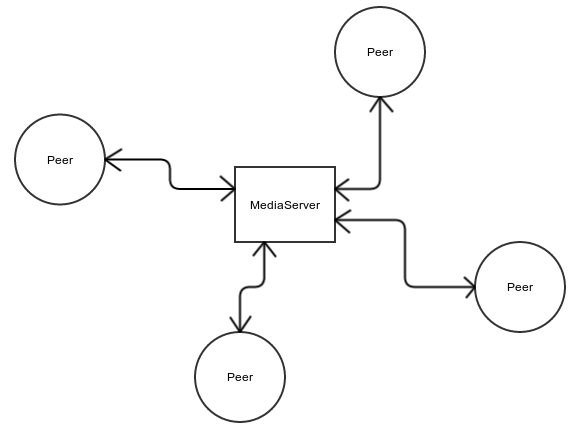
\includegraphics[scale=0.6]{mediaserver.png}
\\
\\
Communication between peers and the media server is done by opening up ports in the firewall to listen for incoming tcp and UDP connections. The media server can receives incoming streams and mix it in with the other streams and forward it to all the other peers. All the streams are identified using an SSRC.

\subsection{Signaling}
Virtual Arena uses a proprietary way of doing signaling over RTCP.

\subsection{Transport}
Raw RTP stream over UDP.

\subsection{Media}
Speex for audio and theora for video.


\section{How does WebRTC work?}
WebRTC is a very complex synergy of components and protocols. But from a frontend developers point of view, all of this is packaged into three main Javascript API's: getUserMedia, RTCPeerConnection and RTCDataChannel. These are defined by the \gls{w3c}. 

The exchange of real-time media between two browsers follows a process like this:

\begin{enumerate}
\item Input devices are opened for capture as the media source. This is done using the getUserMedia API.
\item Now we have to signal the other users that we want to connect to them. using RTCPeerConnection we send an \gls{sdp} offer to the other clients, which generates an \gls{sdp} Answer.The \gls{sdp} here includes \gls{ice} candidates. Which opens ports in the firewall. There is a fallback if both clients are on symmetric \gls{nat}'s and a connection isn't possible to use a \gls{turn} server that acts like a packet mirror, channeling all the packets through the \gls{turn} server.
\item Once connection is successful, a \gls{dtls} connection is opened and all the media from input devices are encoded into packets and transmitted using \gls{srtp}-\gls{dtls} streams.
\item At the destination, the packets are decoded and formatted into a MediaStream.
\item The MediaStream is sent to output devices
\end{enumerate}

\section{What are the differences?}
While Virtual Arena provides a very simple and not so secure solution at the media level. This because in a closed enterprised environemnt this is not needed. Most of the security will lie in the firewall anyways.

But since \gls{wrtc} is a very open solution and is supposed to work with public users firwall configurations, a lot more complex security architecture is needed.

So while \gls{wrtc} packages all their streams in a new format called a MediaStream. At the transport level everything is encrypted using \gls{dtls} on top of \gls{srtp}.

\section{What do we need?}
There are several problems here. Since Virtual Arena operates on a low-level not much is needed. All we need is to listen to a specific ip-address on a specific port on UDP transmitted data. In the packet headers we will find an \gls{ssrc} that we use to identify the incoming packets.

With WebRTC on the other hand, we are only allowed to work on a higher level. We cannot access MediaStreams directly without first opening a connection with another peer. This is a problem. This means that we first have to iniate a normal RTC Connection before we can look at any identifiers such as the \gls{ssrc}. We cannot listen on specific ports for incoming RTC connections, and we cannot specify a specific port to transmit data. Also as of now the current implementation of WebRTC is not designed to add local external streams to the connection. This means that getting WebRTC to work with any external application, we have to create some sort of gateway server.